\documentclass[12pt,fleqn]{article}\usepackage{../common}
\begin{document}
Ders 2

Ornek 

$X \sim N(3,5)$ ise $P(X > 1)$ nedir? Cevap:

\[ P(X>1) = 1 - P(X < 1) = 1 - P( Z < \frac{ 1 - 3}{\sqrt{5 }}) = 
1 - \Phi(-0.8944) = .81
 \]

Soru tam $P(a  < X < b)$, sadece $b$ oldugu icin yukaridaki form ortaya
cikti. 

Ornek 

Simdi oyle bir $q$ bul ki $P(X < q) = .2$ olsun. Yani $\Phi^{-1}(.2)$'yi
bul. Yine $X \sim N(3,5)$. 

Cevap 

Demek ki tablodan $.2$ degerine tekabul eden esik degerini bulup, ustteki
formul uzerinden geriye tercume etmemiz gerekiyor. Normal tablosunda
$\Phi(-0.8416) = .2$, 

\[ .2 = P(X<q) = P( Z < \frac{ q - \mu}{\sigma}) = \Phi(\frac{ q - \mu}{\sigma})
\]

O zaman 

\[ -0.8416 = \frac{q - \mu}{\sigma} = \frac{ q - 3}{\sqrt{ 5}} \]

\[ q = 3 - 0.8416 \sqrt{ 5} = 1.1181 \]

$t$ (Student's t)ve Cauchy Dagilimi 

$X$, $v$ derece bagimsizlikta $t$ dagilimina sahiptir, ki bu $X \sim t_v$
diye yazilir eger 

\[ f(x) = 
\frac{ \Gamma(v+1)/2)} {\sqrt{v\pi}\Gamma(v/2)}
\bigg(1 + \frac{ x^2}{v}\bigg)^{-(v+1)/2}
 \]

$t$ dagilimi Normal dagilima benzer ama daha kuyrugu daha kalindir. Aslinda
Normal dagilimi $t$ dagiliminin $v = \infty$ oldugu hale tekabul
eder. Cauchy dagilimi da $t$'nin ozel bir halidir, $v = 1$ halidir. Bu
durumda yogunluk fonksiyonu

\[ f(x)  = \frac{ 1}{\pi(1+ x^2)} \]

Bu formul hakikaten bir yogunluk mudur? Kontrol icin entegralini alalim, 

\[ \int _{ -\infty}^{\infty} f(x) dx = 
\frac{ 1}{\pi} \int _{ -\infty}^{\infty} \frac{ dx}{1 + x^2} 
 \]

Cogunlukla entegre edilen yerde  ``1 arti ya da eksi bir seyin karesi''
turunde  bir ifade gorulurse, yerine gecirme (subsitution) islemi
trigonometrik  olarak  yapilir. 

\[  x = \tan \theta, \theta = \arctan x \]

\[ 1 + x^2 = 1 + \tan^2\theta = \sec^2\theta\]

\[ dx / d\theta = \sec^2\theta \]

O zaman 

\[ =
\frac{ 1}{\pi} \int _{ -\infty}^{\infty} \frac{ dx}{1 + x^2}   =
\frac{ 1}{\pi} \int _{ -\infty}^{\infty}  \frac{ 1}{\sec^2\theta}\sec^2\theta d\theta = 
\frac{ 1}{\pi} \int _{ -\infty}^{\infty}  1 \ d\theta = 
 \]

\[ = 
\frac{ 1}{\pi} \theta | _{ -\infty}^{\infty}   = 
\frac{ 1}{\pi} [\arctan(\infty) - \arctan(-\infty)]
 \]

\[ =
\frac{ 1}{\pi} [\frac{ \pi}{2} - (-\frac{ \pi}{2}) ] = 1
 \]


$\chi^2$ Dagilimi

$X$'in $p$ derece serbestlige sahip bir $\chi^2$ dagilima sahip ise $X \sim
\chi^2_p$ olarak gosterilir, yogunluk 

\[ f(x) = \frac{ 1}{\Gamma(p/2) 2^{p/2}} x^{(p/2) - 1} e^{-x/2 }, \ x > 0 \]

Eger $Z_1, .. , Z_p$ bagimsiz standart Normal rasgele degiskenler ise,
$\sum _{ i=1}^{p} Z_p \sim \chi^2_p$ esitligi dogrudur. 

Iki Degiskenli Dagilimlar 

Tanim

Surekli ortamda $(X,Y)$ rasgele degiskenleri icin yogunluk fonksiyonu
$f(x,y)$ tanimlanabilir eger i) $f(x,y) > 0, \ \forall (x,y)$ ise, ve ii)
$\int _{ -\infty}^{\infty} \int _{ -\infty}^{\infty} f(x,y) dx dy = 1$ ise ve her kume $A \subset \mathbb{R} \times \mathbb{R}$ icin 
$P((X,Y) \in A) = \int
\int_A f(x,y) dx dy$. Hem ayriksal hem surekli durumda 
birlesik (joint) CDF $F_{X,Y}(x,y) = P (X \le x, Y \le y)$ diye
gosterilir. 

Bu tanimda $A$ kumesi olarak tanimlanan kavram uygulamalarda bir olaya
(event) tekabul eder. Mesela

Ornek

$(X,Y)$'in birim kare uzerinde birbicimli (uniform) olsun. O zaman 

\[ 
f(x,y) =
\left\{ \begin{array}{ll}
1 & \textit{eger} \ 0 \le x \le 1, 0 \le y \le 1 \ ise\\
0 & \textit{diger durumlarda}
\end{array} \right.
 \]

$P(X < 1/2, Y < 1/2)$'yi bul. 

Cevap

Burada verilen $A = \{ X < 1/2, Y < 1/2\}$ bir altkumedir ve bir
olaydir. Olaylari boyle tanimlamamis miydik? Orneklem uzayinin bir
altkumesi olay degil midir? O zaman $f$'i verilen altkume uzerinden entegre
edersek, sonuca ulasmis oluruz. 

Ornek 

Eger dagilim kare olmayan bir bolge uzerinden tanimliysa hesaplar biraz
daha zorlasabilir. $(X,Y)$ yogunlugu 

\[ 
f(x,y) = 
\left\{ \begin{array}{ll}
cx^2y & eger \ x^2 \le y \le 1 \\
0 & digerleri
\end{array} \right.
 \]

Niye $c$ bilinmiyor? Belki problemin modellemesi sirasinda bu bilinmez
olarak ortaya cikmistir. Olabilir. Bu degeri hesaplayabiliriz, cunku
$f(x,y)$ yogunluk olmali, ve yogunluk olmanin sarti $f(x,y)$ entegre
edilince sonucun 1 olmasi. 

Once bir ek bilgi uretelim, eger $x^2 \le 1$ ise, o zaman $-1 \le x \le
1$ 
demektir. Bu lazim cunku entegrale sinir degeri olarak verilecek. 

\[ 1 = \int  \int f(x,y) dy dx = c \int _{ -1}^{1} \int _{ x^2}^{1}x^2y  \]

\[=  c \int _{ -1}^{1} x^2 \int _{ x^2}^{1} y dy dx = 
\int _{ -1}^{1} x^2 (\frac{ 1}{2} - \frac{ x^4}{2} )dx = 1
 \]

\[=  c \int _{ -1}^{1} x^2 (\frac{ 1 - x^4}{2} ) dx = 1 \]

\[ = \frac{ c}{2} \int _{ -1}^{1} x^2 - x^6 dx  = 1\]

Devam edersek $c = 21/4$ buluruz. 

Simdi, diyelim ki bizden $P(X \ge Y)$'yi hesaplamamiz isteniyor. Bu hangi
$A$ bolgesine tekabul eder? Elimizdekiler

\[ -1 \le x \le 1, \  x^2 \le y, \ y \le 1   \]

Simdi bunlara bir de $y \le x$ eklememiz lazim. Yani ortadaki esitsizlige
bir oge daha eklenir.

\[ -1 \le x \le 1 \]

\[  x^2 \le y \le x \]

\[  y \le 1   \]

$x^2 \le y$'yi hayal etmek icin $x^2 = y$'yi dusunelim, bu bir parabol
olarak cizilebilir, ve parabolun ustunde kalanlar otomatik olarak $x^2 \le
y$ 
olur, bu temel irdelemelerden biri. 


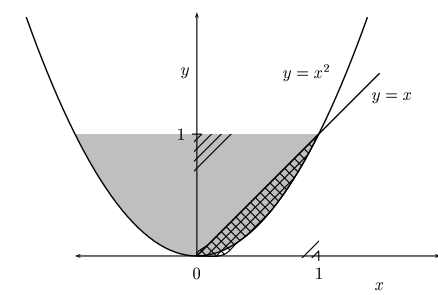
\includegraphics[height=4cm]{2_1.png}

Ayni sekilde $y \le x$ icin $y = x$'i dusunelim, ki bu 45 derece aciyla
cizilmis duz bir cizgi. Cizginin alti $y \le x$ olur. Bu iki bolgenin
kesisimi yukaridaki resimdeki golgeli kisim. 

Ek bir bolge sarti $0 \le x \le 1$. Bu sart resimde bariz goruluyor, ama
cebirsel olarak bakarsak $y \ge x^2$ oldugunu biliyoruz, o zaman $y \ge 0$
cunku $x^2$ muhakkak bir pozitif sayi olmali. Diger yandan $x \ge y$
verilmis, tum bunlari yanyana koyarsak $x \ge 0$ sarti ortaya cikar. 

Artik $P(X \ge Y)$ hesabi icin haziriz, 

\[ P(X \ge Y) = 
\frac{ 21}{4} \int_{ 0}^{1} \int _{ x^2}^{x} x^2y dy dx = 
\frac{ 21}{4} \int_{ 0}^{1} x^2 \bigg[ \int _{ x^2}^{x} y dy \bigg] dx 
 \]

\[ = \frac{ 21}{4} \int _{ 0}^{1} x^2 \frac{ x^2 - x^4}{2} dx = \frac{ 3}{20} \]



\end{document}
